\documentclass[pdftex,12pt,letterpaper]{extarticle}

%%% Set these variables appropriately
%%%
%% Note:  Authors is hardcoded below, this line only used for the PDF info
\newcommand{\AUTHORS}{}
\newcommand{\TITLE}{}
\newcommand{\KEYWORDS}{Put your keywords here}
\newcommand{\CONFERENCE}{Somewhere}
\newcommand{\PAGENUMBERS}{yes}       % "yes" or "no"
\newcommand{\COLOR}{yes}
\newcommand{\showComments}{yes}
\newcommand{\comment}[1]{}
\newcommand{\onlyAbstract}{no}

%%%%%%%%%%%%%%%%%%%%%%%%%%%%%%%%%%%%%%%%%%%%%%%%%%%%%%%%%%%%%%%%%%%%%

%%%
%%%  Page Setup
%%%
\special{papersize=8.5in,11in}
\setlength{\pdfpagewidth}{8.5in}
\setlength{\pdfpageheight}{11in}

\usepackage{ifthen}
\ifthenelse{\equal{\PAGENUMBERS}{yes}}{%
\usepackage[nohead,
            left=1in,right=1in,top=1in,
            footskip=0.5in,bottom=1in,     % Room for page numbers
            columnsep=0.25in
            ]{geometry}
}{%
\usepackage[noheadfoot,left=0.75in,right=0.85in,top=0.75in,
            footskip=0.5in,bottom=1in,
            columnsep=0.25in
	    ]{geometry}
}
\usepackage{mdframed}


%%% Alter some LaTeX defaults for better treatment of figures:
%%% See p.105 of "TeX Unbound" for suggested values.
%%% See pp. 199-200 of Lamport's "LaTeX" book for details.
%%%   General parameters, for ALL pages:
\renewcommand{\topfraction}{0.9}	% max fraction of floats at top
\renewcommand{\bottomfraction}{0.8}	% max fraction of floats at bottom
%%%   Parameters for TEXT pages (not float pages):
\setcounter{topnumber}{2}
\setcounter{bottomnumber}{2}
\setcounter{totalnumber}{4}     % 2 may work better
\setcounter{dbltopnumber}{2}    % for 2-column pages
\renewcommand{\dbltopfraction}{0.99}	% fit big float above 2-col. text
\renewcommand{\textfraction}{0.01}	% allow minimal text w. figs
%%%   Parameters for FLOAT pages (not text pages):
\renewcommand{\floatpagefraction}{0.99}	% require fuller float pages
%%% N.B.: floatpagefraction MUST be less than topfraction !!
\renewcommand{\dblfloatpagefraction}{0.7}	% require fuller float pages


%%%
%%%  Captions
%%%
\usepackage[font=bf]{caption}
%%  Space between figure and caption (assuming caption
%%  is below figure)
%\usepackage[font=bf,aboveskip=0pt]{caption} % SPACE
%%  Space between caption and body text of document
\addtolength{\textfloatsep}{-7pt} % SPACE

%%%
%%%  Section headings
%%%
%\usepackage{titlesec}
%\titlespacing{\paragraph}{0pt}{*1}{*1}      % SPACE
\usepackage[compact]{titlesec}              % SPACE
%\titleformat{\section}%                     % IEEE/ACM: caps + period
%  {\bf\large\uppercase}{\thesection.\quad}{0pt}{}

%%%
%%%  Lists
%%%
\usepackage{enumitem}
\setlist{itemsep=0pt,parsep=0pt}             % more compact lists

%%%
%%%  Header / Footer
%%%
\usepackage{fancyhdr}
\renewcommand{\headrulewidth}{0pt}

\ifthenelse{\equal{\PAGENUMBERS}{yes}}{%
  \pagestyle{plain}
}{%
  \pagestyle{empty}
}

%%%
%%%  Bibliography
%%%
\usepackage[numbers]{natbib}

%%%
%%%  Footnotes / Endnotes
%%%
\interfootnotelinepenalty=10000  % Split footnotes are annoying

% If you want endnodes, uncomment:
%\usepackage{endnotes}
%\usepackage{drafthead}
%\let\footnote=\endnote

%%%
%%%  Tables
%%%
\usepackage{booktabs}
\usepackage{color}
\usepackage{colortbl}
\usepackage{float}                           % Must appear before hyperref to
                                             % avoid weird PDF compile issues

%%%
%%%  Fonts
%%%
\usepackage{mathptmx}                        % Times/Times-like math symbols
\usepackage{courier}
\usepackage[scaled=0.92]{helvet}


%%%
%%% Script letters
%%%
\usepackage[mathscr]{euscript}
\usepackage[T1]{fontenc}
%%%
%%% Code
%%%
\usepackage{listings}
\usepackage{inconsolata}
\definecolor{dkgreen}{rgb}{0,0.6,0}
\definecolor{gray}{rgb}{0.5,0.5,0.5}
\definecolor{mauve}{rgb}{0.58,0,0.82}

\lstset{
	language=C,
	moredelim=**[is][\color{magenta}]{@}{@},
	moredelim=**[is][\color{dkgreen}]{`}{`},
    commentstyle=\color{dkgreen},
  	keywordstyle=\color{blue},
    stringstyle=\color{mauve},
  	numberstyle=\footnotesize\ttfamily\color{gray},
  	basicstyle={\footnotesize\ttfamily},
    breakatwhitespace=false,         
    breaklines=true,                 
    captionpos=b,                    
    keepspaces=true,                 
    numbers=left,                    
    numbersep=5pt,                  
    showspaces=false,                
    showstringspaces=false,
    showtabs=false,                  
    tabsize=2,
	xleftmargin=2em,						% Line numbers inside frame
	framexleftmargin=1.5em,					% Line numbers inside frame
}

% Add extra keywords for code listing here
\lstset{emph = {value\_t, entry\_t, key\_t}, emphstyle = {\color{blue}},%
		emph = {g\_label\_0, g\_label\_1, g\_label\_2, g\_end}, emphstyle = {\color{magenta}}
}
\usepackage[boxruled]{algorithm2e}
\renewcommand{\lstlistingname}{Algorithm}

%%%
%%%  PDF setup
%%%
\ifthenelse{\equal{\COLOR}{yes}}{%
  \usepackage[colorlinks]{hyperref}%         % for online version
}{%
  \usepackage[pdfborder={0 0 0}]{hyperref}%  % for paper (B&W) version
}
\usepackage{url}

\hypersetup{%
pdfauthor = {\AUTHORS},
pdftitle = {\TITLE},
pdfsubject = {\CONFERENCE},
pdfkeywords = {\KEYWORDS},
bookmarksopen = {true}
}

%%
%% Figure placeholder macros
%%
\usepackage[font={small,it}]{subfig}
\definecolor{placeholderbg}{rgb}{0.85,0.85,0.85}
\newcommand{\placeholder}[1]{%
\fcolorbox{black}{placeholderbg}{\parbox[top][1.5in][c]{0.95\columnwidth}{#1}}}


%%%
%%%  Misc
%%%
\usepackage[pdftex]{graphicx}
\usepackage{soul}

%\setlength{\parindent}{0pt}
%\setlength{\parskip}{\baselineskip}

%\clubpenalty=10000  % Don't allow orphans
%\widowpenalty=10000 % Don't allow widows

%%%
%%%  To appear/appeared in text on title page
%%%
\usepackage[absolute]{textpos}
\newcommand{\ToAppear}{%
\begin{textblock*}{\textwidth}(0.95in,0.4in)
\begin{flushright}
    %\noindent{\fbox{\textsf{Under submission---please do not redistribute.}}}
    %  --OR--
    \noindent{\small To appear in \textit{Proceedings of the XYZ}\\
    \noindent{\small \textit{Conference (XYZ'08)}, City, State, Month 2008}}
    %  --OR--
    %\noindent{\small In \textit{Proceedings of the XYZ}\\
    %\noindent{\small \textit{Conference (XYZ'08)}, City, State, Month 2008}}
\end{flushright}
\end{textblock*}
}

%%%
%%%  Sample ACM Copyright Block
%%%
\newfloat{acmcr}{b}{acmcr}
\newcommand{\AcmCopyright}{%
\begin{acmcr}
\parbox[b]{20pc}{%
\footnotesize
Permission to make digital or hard copies of all or part of this work
for personal or classroom use is granted without fee provided that
copies are not made or distributed for profit or commercial advantage
and that copies bear this notice and the full citation on the first
page.  To copy otherwise, to republish, to post on servers or to
redistribute to lists, requires prior specific permission and/or a fee.

{\em Conference}, Month Date--Date, Year, Location\\
Copyright 200X ACM X-XXXXX-XX-X/XX/XX ...\$5.00}
\end{acmcr}}

%%%
%%%  Comments
%%%
%\newcommand{\note}[2]{
%    \ifthenelse{\equal{\showComments}{yes}}{\textcolor{#1}{#2}}{}
%}
\newcommand{\note}[2]{
  \ifthenelse{\equal{\showComments}{yes}}{\textcolor{#1}{\sf\small\fontfamily{phv}\fontseries{mc}\selectfont#2}}{}
}

% Change these to your own initials as you like...
\newcommand{\dga}[1]{\note{blue}{DGA: #1}}
\newcommand{\mk}[1]{\note{red}{MK: #1}}
\newcommand{\dz}[1]{\note{green}{DZ: #1}}
\newcommand{\ak}[1]{\textcolor{red}{#1}}

\date{}
\title{\textbf{\TITLE 15-769 Project\\ User-guided approach to content-based image retrieval}}
\author{{\large Thomas Kim (andrew ID tskim), Conglong Li (andrew ID conglonl)}\\
{\em $\left\{ thomas.kim, conglonl \right\}@cs.cmu.edu$}}


% This needs to be the last thing before \begin{document}
\usepackage{microtype}  % SPACE

%%%%%%%%%%%%%%%%%%%%  START DOCUMENT  %%%%%%%%%%%%%%%%%%%%%%%%
\begin{document}

\maketitle

%\AcmCopyright
%\ToAppear

\section{Introduction}
We propose a system to allow users to provide both negative and positive image queries in order to retrieve images with similar content.
One important application of our system is to allow users to search through their personal photo collections with content-based queries, and as such the
system should not sacrifice performance at smaller scales in order to achieve scalability.
We plan to apply modern machine learning techniques in the context of computer vision to compactly express the content and features of the images, then leverage
this representation to provide efficient querying of the data set.

Evaluation of content-based image retrieval is qualitative, making it difficult to evaluate the success of this system.
As such, the evaluation will be closely tied to qualitative analysis through user studies.
Performance will be evaluated against other state of the art content-based image retrieval systems.

Content-based image retrieval allows retrieval of multimedia data based on the content of the image as opposed to metadata such as text annotations.
In many cases, such annotations are absent or incomplete, necessitating this content-based approach to improve the accuracy and completeness of search results.


%Note: talk about how our system hopes to use a much simpler user interface than approaches like AverageExplorer which are quite complex and poorly suited for mobile.
%Each image in its entirety will be a positive or negative query

\section{Related Work}
\subsection{Content-Based Image Retrieval}
Content-based image retrieval aims at searching for similar images
through the analysis of image content. As DNNs learn rich mid-level
image descriptors, ImageNet uses the feature vectors from the 7th
layer in image retrieval and demonstrated outstanding
performance~\cite{krizhevsky2012imagenet}. Babenko \textit{et al.}
proposed to compress the DNN features using PAC and discriminative
dimensionality reduction to improve the efficiency~\cite{babenko2014neural}.

Due to the recent growth of visual contents, rapid search in a large
database becomes an emerging need. In stead of linear search which has
high computational cost, a practical strategy is to use the technique
of Approximate Nearest Neighbor (ANN) or hashing based method for
speed up~\cite{gionis1999similarity,weiss2009spectral,kulis2009learning,
norouzi2011minimal,liu2012supervised,xia2014supervised}. These methods
project the high-dimensional features to a lower dimensional space, and
then generate the compact binary codes. Benefiting from the produced
binary codes, fast image search can be carried out via binary pattern
matching or Hamming distance measurement. However, these methods require
to use similarity matrix to describe the relationship of the image pairs, which
is no practical for a large-scale dataset. Recently Lin \textit{et al.}
propose an effective deep learning framework to generate binary hash codes
and image representations in a point-wised manner, making it suitable
for large-scale datasets~\cite{lin2015deep}.

\subsection{Image Analysis Applications}
AverageExplorer is an interactive framework that allows an user to rapidly
explore and visualize a large image collection using the medium of average
images~\cite{zhu2014averageexplorer}. This real-time system provides a
way to summarize large amounts of visual data by weighted averages of
an image collection, with the weights reflecting user-indicated importance.
Zhu \textit{et al.} propose a way to help user-controlled realistic image
manipulation by learning the manifold of natural images and defining the
image editing operations with constraints lie on the learned manifold at
all times. Thus the model automatically adjusts the output keeping all edits
as realistic as possible~\cite{zhu2016generative}.

\section{Algorithm}
\label{sec:algo}

\section{Implementation}
\begin{minipage}{1.0\columnwidth}
    \centering
    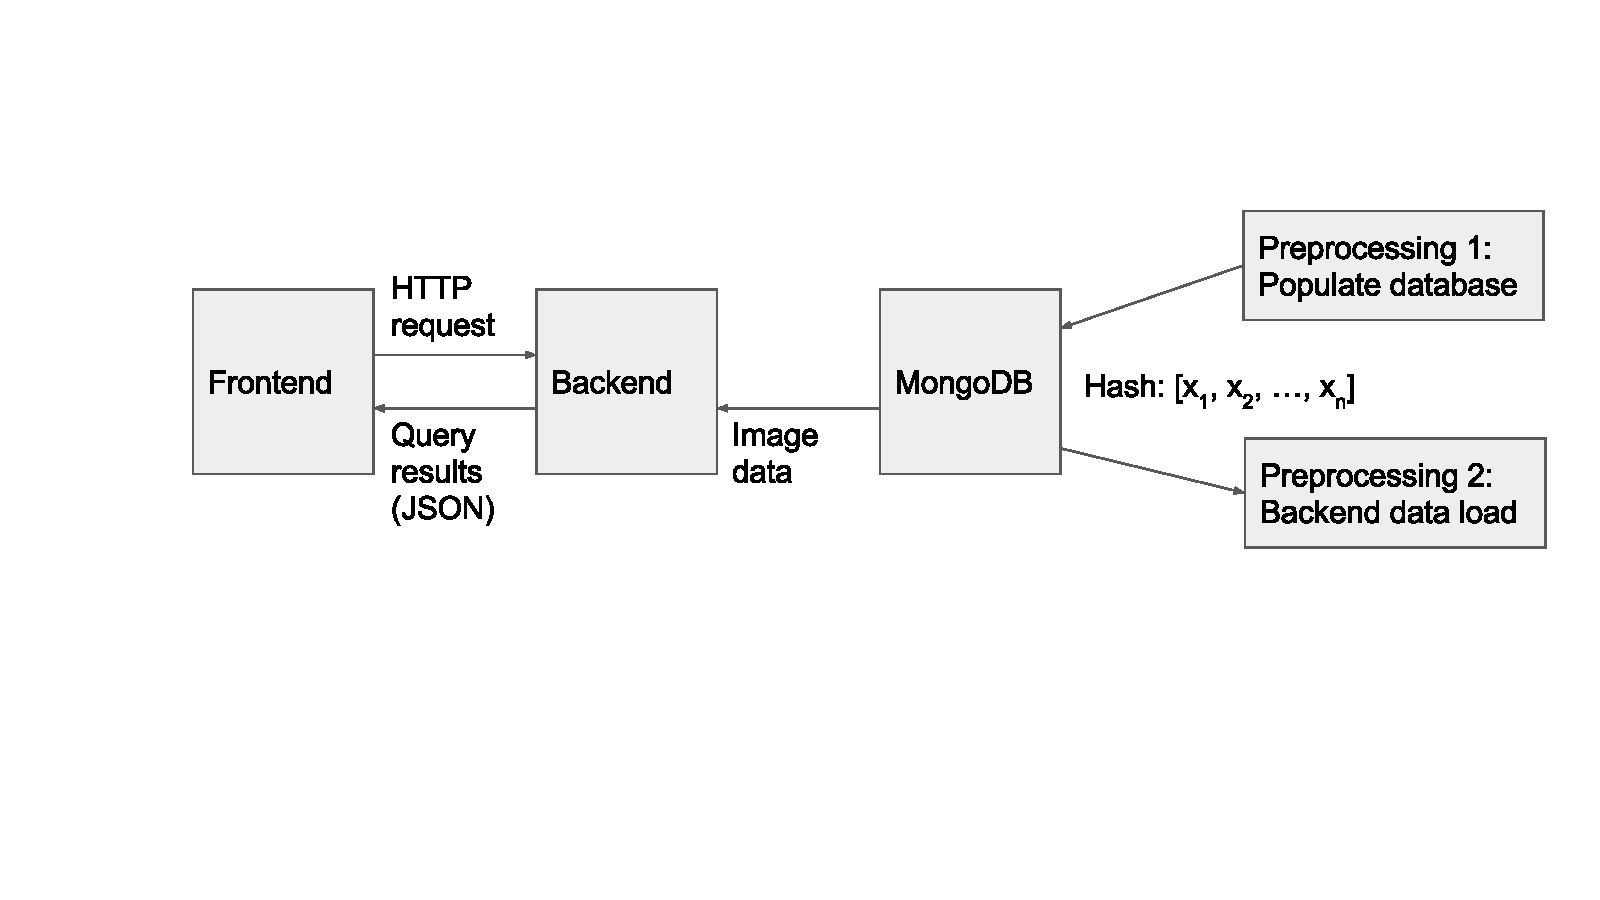
\includegraphics[width=0.9\columnwidth]{figs/system-design}
    \label{system-design}
\end{minipage}
The system works as follows:\\
    1. The frontend sends a series of query images (include and/or exclude) to the backend. \\
    2. The backend calculates the cosine distance from the hash of every query image to the hash of every image in the database.
    3. The backend then hands off these distances to post-processing where the algorithms mentioned in Section \ref{sec:algo}

\subsection{Frontend Design}
The frontend is implemented using Meteor~\cite{coleman2015discover} (special thanks to Michael Kaminsky).
The frontend allows users to see their entire image collection and select images to use as positive
and negative queries by clicking on them.

\subsection{Backend Design}
The backend is implemented in Python and accepts HTTP requests from the frontend.
The backend is persistent and uses a request-based model, rather than invoked upon every new user query,
which is done for performance reasons.
The main mechanism to calculate cosine distances between image hashes is to use the cdist function in the
scipy~\cite{jones2001open} library for Python.

Further work includes optimizing this calculation, as it is currently implemented not as matrix multiplication
but as for loops.
The reason for this seems to be to minimize floating point error, but an application such as this is very
tolerant to rounding and quantization, so we believe there are further performance gains possible on this
operation.

\subsection{Optimizations}
One of the goals of the system was to enable fast (<1s) queries of the image set in order to achieve
a good user experience.
In order to reach this performance goal, we implemented 2 preprocessing steps.
The first preprocessing step uses TensorFlow~\cite{abadi2016tensorflow} to generate hashes for each image and
store them in MongoDB.
The hash in this implementation of imagematch is the output of the pool\_3 layer of the Inception
model~\cite{szegedy2015going} pretrained on the 2012 ImageNet dataset.
Due to time constraints, using other layers was not explored in depth in this project and is left for
future work.
One possible difficulty in using the output of earlier layers is that the amount of memory and computation
increases as the size of the hash increases, and the activations output by earlier layers are larger than
the output of pool\_3.
This preprocessing step takes about TODO hours of CPU time to preprocess 300,000 images.

The second preprocessing step pre-loads all of the hashes from MongoDB into a matrix stored by the backend.
This allows queries to occur without any of the overhead associated with marshalling data into different formats.
This step takes about TODO 120 seconds to complete and is done once every time the dataset changes.

\section{Evaluation}
The evaluation of the query result quality and the performance were done completely separately.
The former was done using user studies and on a hand-picked image set (dataset 1), while the latter was done
on an arbitrarily chosen subset of the ImageNet dataset\cite{krizhevsky2012imagenet} (dataset 2).

Dataset 1 is of modest size (about 150 images), whereas dataset 2 varies in size from 10,000 to 300,000 images.
Due to time constraints, image sets larger than 300,000 images were left for future work.

\section{Summary}


%\appendix
%\input{appendix_sources}

%\vspace{-0.1in}
%\section*{Acknowledgments}
% Comments for people we need to ack in the final version

\bibliography{ref}
\bibliographystyle{abbrvnat}

\end{document}

% Local Variables:
% TeX-command-default: "LaTeX PDF"
% End:

